\documentclass{article}


\usepackage{1}

\usepackage[utf8]{inputenc} % allow utf-8 input
\usepackage[T1]{fontenc}    % use 8-bit T1 fonts
\usepackage{hyperref}       % hyperlinks
\usepackage{url}            % simple URL typesetting
\usepackage{booktabs}       % professional-quality tables
\usepackage{amsfonts}       % blackboard math symbols
\usepackage{nicefrac}       % compact symbols for 1/2, etc.
\usepackage{microtype}      % microtypography
\usepackage{lipsum}		% Can be removed after putting
\usepackage{xcolor}
\usepackage{cite}
\usepackage{tikz}
\usepackage{appendix}
\usetikzlibrary{chains,scopes,shapes.geometric}
\usepackage{amsmath}
\usepackage{amssymb}
\usepackage{booktabs} 
\usepackage{multirow}
\usepackage{indentfirst}
\usepackage{lipsum}
\usepackage{amsfonts}
\usepackage{epstopdf}
\usepackage{algorithmicx}
\usepackage{ntheorem}
%\usepackage{algorithm}
\usepackage{float}
\usepackage{enumitem}
\let\algorithm\relax  

\let\endalgorithm\relax  
\newtheorem{theorem}{Theorem}
\newtheorem{lemma}{Lemma}
%\newtheorem{proof}{Proof}[section]
\newtheorem*{Proof}{Proof}
\usepackage[linesnumbered,ruled,vlined]{algorithm2e}{  
	\usepackage{algpseudocode}
	
	\newcommand\ldq\textquotedblleft
	\newcommand\rdq\textquotedblright{}
	\newcommand\mb\mathbb
	\newcommand\mf\mathbf
	\newcommand\tf\textbf

	\renewcommand{\algorithmicrequire}{\textbf{Input:}}  % Use Input in the format of Algorithm  
	\renewcommand{\algorithmicensure}{\textbf{Output:}} % Use Output in the format of Algorithm   
	
\title{Numerical Solver for MAC Scheme Stokes Equation }
\date{January, 2021}	% Here you can change the date presented in the paper title
%\date{} 					% Or removing it

\author{
  Ruicheng Ao\\
  School of Mathematical Sciences\\
  Peking University\\

  \texttt{archer\_arc@pku.edu.cn} \\
  %% examples of more authors
 \\
  %% \AND
  %% Coauthor \\
  %% Affiliation \\
  %% Address \\
  %% \texttt{email} \\
  %% \And
  %% Coauthor \\
  %% Affiliation \\
  %% Address \\
  %% \texttt{email} \\
  %% \And
  %% Coauthor \\
  %% Affiliation \\
  %% Address \\
  %% \texttt{email} \\
}

\begin{document}
\maketitle


In this report, we consider Stokes equation:
$$\begin{aligned}
	-\Delta \vec{u}+\nabla{p} &= \vec{F}, \\
	div{\vec{u}}& = 0,\\
	\frac{\partial{u}}{\partial{\tf{v}}} = b,y = 0&;\frac{\partial{u}}{\partial{\tf{v}}} = t,y = 1,\\
	\frac{\partial{v}}{\partial{\tf{v}}} = l,x=0&;\frac{\partial{v}}{\partial{\tf{v}}} = r,x=1,\\
	u = 0, x=0,1&; v = 0,y=0,1,
	\end{aligned}$$
	with velocity $\vec{u}=(u,v)$, pressure $p$, external force $\vec{F} = (f,g)$ and outer normal direction $\tf{v}$. The domain given is $\Omega = (0,1)\times(0,1)$. We suggest the solution is 
	$$ \left\{
		\begin{aligned} 
		u &= (1-\cos{(2\pi x)})sin{(2\pi y)},\\
		v &= -(1-\cos{(2\pi y)})sin{(2\pi x)}.
		\end{aligned}\right.
		$$ It follows that 
		$$\left\{\begin{aligned}
			f(x,y) &= -4\pi^2(2\cos{(2\pi x)}-1)\sin{(2\pi y)}+x^2,\\
			g(x,y) & = 4\pi^2(2\cos{(2\pi y)}-1)\sin{(2\pi x)}.
		\end{aligned}
		\right.$$




\section{Numerical Scheme}
We rewrite the Stokes equations into coordinate-wise:
 \begin{eqnarray}
	-\Delta{u} + \partial_x{p} = f, \\
	-\Delta{v} +\partial_y{p}  =g, \\
	-\partial_x{u}-\partial_y{v} = Div.
\end{eqnarray} 
The MAC scheme is to discretize the x-coordinate momentum equation (1) at vertical edges, the y-coordinate momentum equation (2) at horizontal edges, and the continuity equation (3) at cell centers using central difference schemes. For grid of size $N$, let $h=1/N$. We denote by
$$\begin{aligned}
f_{i,j} = f(ih,(j-0.5)h), 1\le i\le N-1,1\le j\le N;&\quad g_{i,j} = g((i-0.5)h,jh),1\le i\le N,1\le j\le N-1;\\
b_i = b(ih),t_i = t(ih),1\le i\le N-1;&\quad l_j=l(ih),r_j=r(jh),1\le j\le N-1;\\
u_{i,j} = u(ih,(j-0.5)h),0\le i\le N,1\le j\le N;&\quad v_{i,j} = v((i-0.5)h,jh),1\le i\le N,0\le j\le N;\\
p_{i,j} = p((i-0.5)h,(j-0.5)h),1\le i\le N,1\le j\le N.
\end{aligned}$$
\begin{center}
	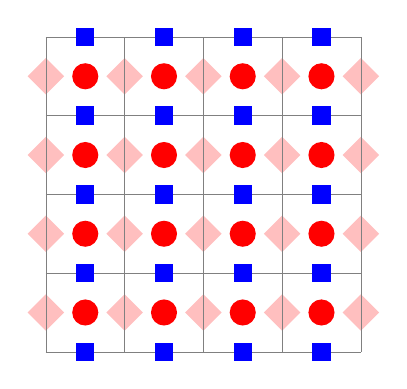
\begin{tikzpicture}
%	\draw (2,2) -- (-2,2) -- (-2,-2) -- (2,-2) -- cycle;
	\draw[step=1,help lines] ( -2,-2 ) grid (2, 2); 
	\foreach \x in {-2,...,2}{
	    \foreach \y in {-1.5,...,1.5} {
		\node at(\x,\y)[shape=diamond,draw = none,fill=pink,draw opacity=0]{};
	}}
	\draw[step=1,help lines] ( -2,-2 ) grid (2, 2); 
	\foreach \y in {-2,...,2}{
	\foreach \x in {-1.5,...,1.5} {
		\node at(\x,\y)[shape = rectangle, draw = none, fill = blue]{};
}}
	\foreach \y in {-1.5,...,1.5}{
	\foreach \x in {-1.5,...,1.5} {
		\node at(\x,\y)[shape = circle, draw = none,fill = red] {};
}}
	\end{tikzpicture}
\end{center}
See the figure. Using central difference scheme we have the following equations:
$$\begin{aligned}
	\frac{3u_{i,j}}{h^2}-\frac{u_{i-1,j}}{h^2}-\frac{u_{i+1,j}}{h^2}-\frac{u_{i,j+1}}{h^2}-(\frac{p_{i,j}}{h}-\frac{p_{i+1}}{h}) &= f_{i,j}+\frac{b_i}{h},\quad 1\le i\le N-1,j=1;\\
		\frac{4u_{i,j}}{h^2}-\frac{u_{i-1,j}}{h^2}-\frac{u_{i+1,j}}{h^2}-\frac{u_{i,j+1}}{h^2}-(\frac{p_{i,j}}{h}-\frac{p_{i+1}}{h}) &= f_{i,j},\quad 1\le i\le N-1,2\le j\le N-1;\\
		\frac{3u_{i,j}}{h^2}-\frac{u_{i-1,j}}{h^2}-\frac{u_{i+1,j}}{h^2}-\frac{u_{i,j+1}}{h^2}-(\frac{p_{i,j}}{h}-\frac{p_{i+1}}{h}) &= f_{i,j}+\frac{t_i}{h},\quad 1\le i\le N-1,j=N\\
		u_{0,j} = u_{N,j} &= 0,\quad 1\le j\le N;\\
		\frac{3v_{i,j}}{h^2}-\frac{v_{i+1,j}}{h^2}-\frac{v_{i,j-1}}{h^2}-\frac{v_{i,j+1}}{h^2} -(\frac{p_{i,j}}{h}-\frac{p_{i,j+1}}{h})&= g_{i,j}+\frac{l_j}{h},\quad i=1,1\le j\le N-1;\\
	\frac{4v_{i,j}}{h^2}-\frac{v_{i+1,j}}{h^2}-\frac{v_{i,j-1}}{h^2}-\frac{v_{i,j+1}}{h^2} -(\frac{p_{i,j}}{h}-\frac{p_{i,j+1}}{h})&= g_{i,j},\quad 2\le i\le N-1,1\le j\le N-1;\\
	\frac{3v_{i,j}}{h^2}-\frac{v_{i+1,j}}{h^2}-\frac{v_{i,j-1}}{h^2}-\frac{v_{i,j+1}}{h^2} -(\frac{p_{i,j}}{h}-\frac{p_{i,j+1}}{h})&= g_{i,j}+\frac{r_j}{h},\quad i=N,1\le j\le N-1;\\
	v_{i,0} = v{i,N} &= 0,\quad 1\le i\le N;\\
	\frac{u_{i-1,j}}{h}-\frac{u_{i,j}}{h}+\frac{v_{i,j-1}}{h}-\frac{v_{i,j}}{h} &= Div_{i,j},\quad 1\le i\le N, 1\le j\le N.
\end{aligned}$$
It can be written as matrix form
\begin{eqnarray} \label{eqn:stokes}
	\begin{bmatrix}
		A &B\\
		B^T& 0
	\end{bmatrix}
	\begin{bmatrix}
	U\\
	P
	\end{bmatrix}
	=\begin{bmatrix}
		F\\Div
	\end{bmatrix},
\end{eqnarray}
where 
$$
A = \begin{bmatrix}
 	\frac{1}{h^2}T_1 & -\frac{1}{h^2}I &&&&&&&&\\
 	-\frac{1}{h^2}I & \frac{1}{h^2}T_2 &-\frac{1}{h^2}I&&&&&&&\\
 	&\ddots&\ddots&\ddots&&&&&&\\
 	&&-\frac{1}{h^2}I&\frac{1}{h^2}T_2&-\frac{1}{h^2}I&&&&&\\
 	&&&-\frac{1}{h^2}I&\frac{1}{h^2}T_1&&&&&\\
 &&&&&	\frac{1}{h^2}T_3&-\frac{1}{h^2}I&&&\\
 &&&&& -\frac{1}{h^2}I&\frac{1}{h^2}T_3&-\frac{1}{h^2}I&&\\
 &&&&&&\ddots&\ddots&\ddots&\\
&&&&&&&-\frac{1}{h^2}I&\frac{1}{h^2}T_3&-\frac{1}{h^2}I\\
   & & && & & & &-\frac{1}{h^2}I &\frac{1}{h^2}T_3
\end{bmatrix},$$
$$
B = \begin{bmatrix}
	-\frac{1}{h}D & &&\\
	&\ddots&&\\
	&&\ddots&\\
	&&&-\frac{1}{h}D\\
	-\frac{1}{h}I&\frac{1}{h}I&&\\
	&\ddots&\ddots&\\
	&&-\frac{1}{h}I&\frac{1}{h}I
\end{bmatrix},$$
and submatrix 
$$
T_1 = \begin{bmatrix}
	3&-1 &&&\\
	-1&3&-1&&\\
	&\ddots&\ddots&\ddots&\\
	&&-1&3&-1\\
	&&&-1&3
\end{bmatrix},
T_2 = \begin{bmatrix}
	4&-1&&&\\
	-1&4&-1&&\\
	&\ddots&\ddots&\ddots&\\
	&&-1&4&1\\
	&&&-1&4
\end{bmatrix},
$$
$$T_3 = \begin{bmatrix}
 3&-1&&&\\
 -1&4&-1&&\\
 &\ddots&\ddots&\ddots&\\
 &&-1&4&-1\\
 &&&-1&3
\end{bmatrix},
D = \begin{bmatrix}
-1&1&&&\\
&-1&1&&\\
&&\ddots&\ddots&\\
&&&-1&1
\end{bmatrix},$$
and $I$ is the $N-1$ order identity. Here 
$$\begin{aligned}
U&=(u_{1,1},\dots,u_{N-1,1},\dots,u_{N-1,N},v_{1,1},\dots,v_{1,N-1},\dots,v_{N,N-1})^T,\\
P &= (p_{1,1},\dots,p_{N,1},\dots,p_{N,N})^T,\\
F&=(\tilde{f}_{1,1},\dots,\tilde{f}_{N-1,1},\dots,\tilde{f}_{N-1,N},\tilde{g}_{1,1},\dots,\tilde{g}_{1,N-1},\dots,\tilde{g}_{N,N-1})^T\end{aligned},
$$
$$\tilde{f}_{i,j} = \left\{  \begin{aligned}
&f_{i,j}+\frac{b_i}{h},\quad j=1\\
&f_{i,j}, \quad 2\le j\le N\\
&f_{i,j}+\frac{t_i}{h},\quad j=N
\end{aligned},\quad \right. \tilde{g}_{i,j} = \left\{ \begin{aligned}
	&g_{i,j}+\frac{l_j}{h},\quad i=1\\
	&g_{i,j},\quad 2\le i\le N-1\\
	&g_{i,j}+\frac{r_j}{h}, \quad i = N
\end{aligned} \right.
$$
We have the following theorem:
\begin{theorem}\label{B}
	The spectral of $B^TA^{-1}B$ consist of $0$s and $1$s.
\end{theorem}
\begin{Proof}
	The proof is left in appendix.
\end{Proof}

\section{Distributive Gauss Seidel}
This section is based on 2020 fall's numerical linear algebra lecture  and Long Chen's paper\cite{wang2013multigrid}.
\subsection{Algorithm Analysis}
Since the matrix in (\ref{eqn:stokes}) is not diagonally dominant, and the zeros block in the diagonal hampers the relaxation, we use distributive relaxation instead. To speak specifically, denote by 
$$L = \begin{bmatrix}
 A&B\\B^T&0
\end{bmatrix},\quad M = \begin{bmatrix}
 I & B\\ 0 & -B^TB
\end{bmatrix}.$$
We have $$LM= \begin{bmatrix}
 A& AB-BB^TB\\B^T &B^TB
\end{bmatrix} \approx \begin{bmatrix}
 A&0\\B^T&B^TB
\end{bmatrix} := \widetilde{LM}.$$
Let $A_p = B^TB$ and $\tilde{A},\tilde{A_p}$ be approximation of $A,A_p$, respectivelly, then the DGS algorithm is given as following.\\
\begin{algorithm}[H]\label{alg:DGS}
		\caption{Distributive Gauss Seidel}
		Relax the momentum equation
		$$U^{k+\frac{1}{2}} = U^k + \widetilde{A^{-1}}(F-AU^k-BP^k).$$\\
		Relax the transformed mass equation
		$$\delta = \widetilde{A_p^{-1}}(Div - BU^{k+\frac{1}{2}}).$$\\
		Distribute the correction to the original varibales
		$$ \begin{aligned}
			U^{k+1} &= U^{k+\frac{1}{2}} + B\delta,\\
			P^{k+1} &= P^k -A_p\delta. 
		\end{aligned}$$\\
\end{algorithm}
To implement it in Matlab, we can write the code by steps below.
\begin{itemize}
	\item[(1)] Using $U^k$ as initial value, do one GS iteration for $AU=F-BP^k$ to get $U^{k+\frac{1}{2}}.$ We notice that there is no need to compute $A^{-1}$ and it is convenient to update one-by-one. For example, the update for velocity $u_{i,j}$ for $i = 1,\dots,N-1,j = 2,\dots,N-1$ can be simply written as
	$$ u_{i,j} = (h^2*\tilde{f}_{i,j}-h*(p_{i+1,j}-p_{i,j})+u_{i-1,j}+u_{i+1,j}+u_{i,j-1}+u_{i,j+1})/4,$$
	and the coefficient 4 should be changed to 3 for $u$ near the bottom or top edges accordingly. The fomula is similar for $v$.
	\item[(2)] Compute divergence residual for internal grids and update the velocity and pressure. This is the same as in V-cycle lecture. Say
	$$ r = -\frac{u_{i,j}-u_{i-1,j}}{h}-\frac{v_{i,j}-v_{i,j-1}}{h}+Div_{i,j},$$
		here $Div$ is the divergence. Let $\delta = r*h/4$, we update velocity and pressure
		$$\begin{aligned}
u_{i,j} &= u_{i,j}+\delta\\
u_{i-1,j} & = u_{i_1,j}-\delta\\
v_{i,j} & = v_{i,j}+\delta\\
v_{i,j-1} &= v_{i,j-1}-\delta \\
		p_{i,j} &= p_{i,j} +r\\
p_{i+1,j}& = p_{i+1,j}-r/4\\
p_{i-1,j} & =p_{i-1,j} -r/4\\
p_{i,j-1} & =p_{i,j-1}-r/4\\
p_{i,j+1}&=p_{i,j+1}-r/4 
		\end{aligned} \\
		$$
	\item[(3)] Compute divergence residual for grids on edges and update the velocity and pressure. This is similar to that above, except that we should replace $4$ with $3$ and do not change velocity on edges and pressure outside the domain.
	\item[(4)] Compute divergence residual for grids on corners and update the velocity and pressure. This is almost the same except that we have to replace $4$  with $2$. 
	\item[(5)] After the update above, we get $U^{k+1}$ and $P^{k+1}$.
\end{itemize}
The convergence analysis could be found in Chen's lecture\cite{chenfinite}. We omit it here for simplicity.
\subsection{V-cycle mutigrid}
Consider the equation $$\begin{bmatrix} 
 A_h &B_h \\ B_h^T &0 
\end{bmatrix}\begin{bmatrix}
 \tilde{U}_h \\ \tilde{P}_h 
\end{bmatrix}= \begin{bmatrix}
 \tilde{F}_h \\ \tilde{Div}_h
\end{bmatrix}.
$$
The V-cycle multigrid algorithm is described as followsing:
\begin{itemize}
	\item[(1)] On grid $\Omega^h$, using $U_h^0,P_h^0$ as initial value, presmooth by DGS for $n_1$ times. Compute the residual $rF_h = F_h -A_hU_h^{n_1}-B_hP_h^{n_1},rDiv_h = Div_h-B_h^TU_h^{n_1}$.
	\item[(2)] Restrict the residual to the coarse grid.
	\item[(3)]Using $U_{2h}^0,P_{2h}^0=0$ as initial values, presmooth 
	$$\begin{bmatrix}
	A_{2h}&B_{2h}\\B_{2h}^T&0 
	\end{bmatrix}\begin{bmatrix}
	 U_{2h} \\ P_{2h}
	\end{bmatrix} = \begin{bmatrix}
	 F_{2h}\\Div_{2h}
	\end{bmatrix}.$$
	by DGS for $n_1$ times. Compute the residual $rF_{2h}= F_{2h}-A_{2h}U_{2h}^{n_1}-B_{2h}P_{2h}^{n_1},rDiv_{2h} = Div_{2h}-B_{2h}^TU_{2h}^{n_1}.$ 
	\item[(4)] Restrict the residual to the coarse grid.
	\item[(5)] Recursively use the steps above until grid $\Omega_{Lh}$. Iterate DGS on $\Omega_{Lh}$ till converge. We get $P_{Lh} = B_{Lh}^TA_{Lh}^{-1}F_{Lh}-D_{Lh}, U_{Lh} = A_{Lh}^{-1}(F_{Lh}-B_{Lh}P_{Lh}).$
	\item[(6)] Prolongate the correction to the fine grid. Using the corrected $U,P$ as inital values, iterate with DGS for $n_2$times to get $U^{n_1+n_2},P^{n_1+n_2}$.
	\item[(7)] Continue this prolongation process until it comes to $\Omega_h$. If the residual on $\Omega_h$ is smaller than toleration, the algorithm terminates. Otherwise restart from step 1 with $U,P$ we've just got.
\end{itemize}
The restriction operators are
$$ R_{h,2h}^u = \frac{1}{8}\begin{bmatrix}
1&2&1 \\ &*& \\ 1&2&1
\end{bmatrix}, R_{h,2h}^v = \frac{1}{8}\begin{bmatrix}
1 & & 1\\ 2 &*& 2\\ 1 & & 1
\end{bmatrix}, R_{h,2h}^p = \frac{1}{4}\begin{bmatrix}
1 & & 1\\ & * & \\ 1& & 1
\end{bmatrix}.  $$
Using figures we can get it more easily.
\begin{center}
	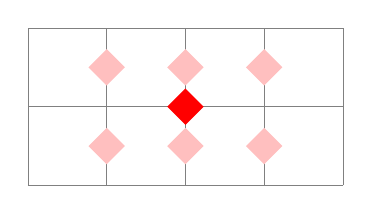
\begin{tikzpicture}
	%	\draw (2,1) -- (-2,1) -- (-2,-1) -- (2,-1) -- cycle;
	\draw[step=1,help lines] ( -2,-1 ) grid (2, 1); 
	\foreach \x in {-1,...,1}{
		\foreach \y in {-0.5,0.5} {
			\node at(\x,\y)[shape=diamond,draw = none,fill=pink]{};
	}}
	\node at(0,0)[shape=diamond,draw = none, fill = red]{};
	\end{tikzpicture}
		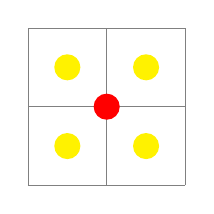
\begin{tikzpicture}
	%	\draw (2,1) -- (-2,1) -- (-2,-1) -- (2,-1) -- cycle;
	\draw[step=1,help lines] ( -1+4,-1 ) grid (1+4, 1); 
	\foreach \x in {-0.5+4,0.5+4}{
		\foreach \y in {-0.5,0.5} {
			\node at(\x,\y)[shape=circle,draw = none,fill=yellow]{};
	}}
	\node at(4,0)[shape=circle,draw = none, fill = red]{};
	\end{tikzpicture}
\end{center}
The red point is the weighted average of the nearest points. For $u$, the weights of upper and lower point are twice of those on the corners. It is similar for $v$. For $p$ it is just the average of the four nearest points.  
For the prolongation operators, we typically apply bilinear interpolation of neighboring coarse-grid unknowns in the staggerd grid. See the figure below.
\begin{center}
		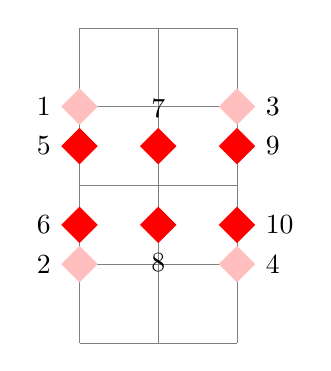
\begin{tikzpicture}
	%	\draw (-1,4 -- (-2,1) -- (-2,-1) -- (2,-1) -- cycle;
	\draw[step=1,help lines] ( -1,-2 ) grid (1, 2); 
			\node at(-1,1)[shape=diamond,draw = none,fill=pink,label = left:1]{};
			\node at(1,1)[shape=diamond,draw = none,fill=pink,label = right:3]{};
			\node at(1,-1)[shape=diamond,draw = none,fill=pink,label = right:4]{};
			\node at(-1,-1)[shape=diamond,draw = none,fill=pink,label = left:2]{};
			\node at(-1,0.5)[shape=diamond,draw = none,fill=red,label = left:5]{};
			\node at(-1,-0.5)[shape=diamond,draw = none,fill=red,label = left:6]{};	
			\node at(0,0.5)[shape=diamond,draw = none,fill=red,label = 7]{};	
			\node at(0,-0.5)[shape=diamond,draw = none,fill=red,label = below:8]{};	
			\node at(1,0.5)[shape=diamond,draw = none,fill=red,label = right:9]{};
			\node at(1,-0.5)[shape=diamond,draw = none,fill=red,label = right:10]{};
	\end{tikzpicture}
\end{center}
We have $u_5 = \frac{3}{4}u_1+\frac{1}{4}u_2,u_6 = \frac{1}{4}u_1+\frac{3}{4}u_2,u_9 = \frac{3}{4}u_3+\frac{1}{4}u_4,u_{10}=\frac{3}{4}u_4+\frac{1}{4}u_3,u_7=\frac{1}{2}(u_5+u_9),u_8 = \frac{1}{2}(u_6+u_{10}).$ The transformation is similar for $v$. And for $p$, we just use the nearest point's value. Finally, let velocity on edges be $0$. 
\subsection{Numerical Results}
Using DGS smoothing with Vcycle multigrid method, choose $\frac{||r_h||_2}{||r_0||_2} \le 10^{-8}$ as stop criteria. For initial value $U^0 = 0,P^0 = 0$ and different $n_1,n_2,L$, we have experimental results below.
		\begin{table}

	\centerline{
		\begin{tabular}{|c|c|c|c|c|}
			\hline
			\multicolumn{5}{|c|}{$L = N/2$}\\
			\cline{1-5}
			N & $n_1,n_2$ & V-cycle times  &CPU time(s)& err \\
			\hline
			\multirow{5}*{64}	& 1,1 &  31 &  0.0642& 0.0015\\
			\cline{2-5}
			& 2,2& 22&0.0719 &0.0015\\
			\cline{2-5}
			& 2,3& 20& 0.0809&0.0015\\
			\cline{2-5}
			&3,3 & 18& 0.0834&0.0015\\
			\cline{2-5}
			& 2,4& 18&0.0757&0.0015\\
			\cline{1-5}
			\multirow{5}*{128}	& 1,1 &  35 &  0.2451& 3.7363e-04\\
			\cline{2-5}
			& 2,2&26 & 0.2853&3.7363e-04\\
			\cline{2-5}
			& 2,3& 23& 0.2743&3.7363e-04\\
			\cline{2-5}
			&3,3 & 21& 0.2973&3.7363e-04\\
			\cline{2-5}
			& 2,4&21 & 0.2971&3.7363e-04\\	
			\cline{1-5}
			\multirow{5}*{256}	& 1,1 &  40 &  1.0337& 9.3398e-05\\
			\cline{2-5}
			& 2,2&30 & 1.3024&9.3398e-05\\
			\cline{2-5}
			& 2,3&26 & 1.1680&9.3398e-05\\
			\cline{2-5}
			&3,3 &24 &1.1654 &9.3398e-05\\
			\cline{2-5}
			& 2,4& 24& 1.3912&9.3398e-05\\	
			\cline{1-5}
			
			\multirow{5}*{512}	& 1,1 &  45 &  7.3908& 2.3349e-05\\
			\cline{2-5}
			& 2,2&33 & 8.2950&2.3349e-05\\
			\cline{2-5}
			& 2,3&30 & 8.7525 &2.3349e-05\\
			\cline{2-5}
			&3,3 & 27&9.5431&2.3349e-05\\
			\cline{2-5}
			& 2,4& 27&9.0193 &2.3349e-05\\	
			\hline	
			\multirow{5}*{1024}	& 1,1 &  49 &  37.2065& 5.8372e-06\\
			\cline{2-5}
			& 2,2& 37& 46.8557& 5.8372e-06\\
			\cline{2-5}
			& 2,3&33 & 51.8100&5.8372e-06\\
			\cline{2-5}
			&3,3 & 30& 54.8474&5.8372e-06\\
			\cline{2-5}
			& 2,4&29 & 51.2733&5.8372e-06\\	
			\hline
			\multirow{5}*{2048}	& 1,1 &  53 &  186.3297& 1.4593e-06\\
			\cline{2-5}
			& 2,2& 40& 227.5852&1.4593e-06\\
			\cline{2-5}
			& 2,3& 36&248.9021 & 1.4593e-06\\
			\cline{2-5}
			&3,3 & 32&253.3137 &1.4593e-06\\
			\cline{2-5}
			& 2,4&32  &258.0706 &1.4593e-06\\
			\hline
\end{tabular} }
						\caption{numerical results for DGS when $L=N/4$}
 \end{table}
		\begin{table}
	\centerline{
		\begin{tabular}{|c|c|c|c|c|}
			\hline
			  \multicolumn{5}{|c|}{$L = N/4$}\\
			\cline{1-5}      
			N & $n_1,n_2$ & V-cycle times  &CPU time(s)& err \\
			\hline
			\multirow{5}*{64}	& 1,1 &  30 &  0.0790& 0.0015\\
			\cline{2-5}
			& 2,2& 22& 0.0724&0.0015\\
			 			\cline{2-5}
			 						& 2,3& 20& 0.0868& 0.0015\\
			 			\cline{2-5}
			 						&3,3 &18 &0.0783 &0.0015\\
			 			\cline{2-5}
			& 2,4& 18& 0.0750&0.0015\\
			\cline{1-5}
			\multirow{5}*{128}	& 1,1 & 36 &  0.2476& 3.7363e-04\\
\cline{2-5}
& 2,2& 26&0.2556 &3.7363e-04\\
\cline{2-5}
& 2,3& 23& 0.2495&3.7363e-04\\
\cline{2-5}
&3,3 &21 & 0.2587 &3.7363e-04\\
\cline{2-5}
& 2,4& 21& 0.3295&3.7363e-04\\	
\cline{1-5}
\multirow{5}*{256}	& 1,1 &  40&  0.9557& 9.3398e-05\\
\cline{2-5}
& 2,2& 30& 1.1379&9.3398e-05\\
\cline{2-5}
& 2,3&26 & 1.1035&9.3398e-05\\
\cline{2-5}
&3,3 & 24&1.3206 &9.3398e-05\\
\cline{2-5}
& 2,4&24 & 1.1006&9.3398e-05\\	
\cline{1-5}
		\multirow{5}*{512}	& 1,1 &45   & 6.3221& 2.3349e-05\\
\cline{2-5}
& 2,2& 33&7.6550 &2.3349e-05\\
\cline{2-5}
& 2,3&29 & 7.7562&2.3349e-05\\
\cline{2-5}
&3,3 &27 & 8.1303&2.3349e-05\\
\cline{2-5}
& 2,4& 27& 8.7585&2.3349e-05\\	
\hline	
\end{tabular} } 

\end{table}
\begin{table}
\centerline{
\begin{tabular}{|c|c|c|c|c|}
\hline
\multicolumn{5}{|c|}{$L = N/4$}\\
\cline{1-5}      
N & $n_1,n_2$ & V-cycle times  &CPU time(s)& err \\
\hline
	\multirow{5}*{1024}	& 1,1 & 50  &  34.4578& 5.8372e-06\\
\cline{2-5}
& 2,2&37 &44.1880  &5.8372e-06\\
\cline{2-5}
& 2,3&32 & 46.8784&5.8372e-06\\
\cline{2-5}
&3,3 & 29& 52.0154&5.8372e-06\\
\cline{2-5}
& 2,4&29 &46.6444 &5.8372e-06\\
\hline
		\multirow{5}*{2048}	& 1,1 &  54 &  167.5138& 1.4593e-06\\
\cline{2-5}
& 2,2& 40& 215.7680&1.4593e-06\\
\cline{2-5}
& 2,3& 35&226.3154 &1.4593e-06\\
\cline{2-5}
&3,3 & 32& 249.8871&1.4593e-06\\
\cline{2-5}
& 2,4&32 & 254.8948&1.4593e-06\\
			\hline
			
	\end{tabular} } 		\caption{numerical results for DGS when $L=N/2$}\end{table}

We can see that, the CPU time cost is nearly $O(n^2)$ and of course V-cycle times decrease as $n_1,n_2$ increase. However, as the number of smoothing increases on each grid, the time consumption increases for one cycle. For this reason, it is better to use fewer smoothing operators for large $N$. Since our stop criteria is the same, the differences between errors are tiny. But for larger $L$, the bottom grid is croaser and the cost of accurate solution on this grid is lower, though it increases the number of prolongation and makes the solution more imprecise. Finally, because of the difference scheme's errors, when $N$ is larger, the error between discrete solution and true solution is smaller.

\section{Uzawa}
\subsection{Algorithm Analysis}
Consider the equation 
$$ SP = \widetilde{Div},$$
where $S=B^TA^{-1}B$ and $\widetilde{Div}=B^TA^{-f}F-Div$. This is otained from equation (\ref{eqn:stokes}) by eliminating $u$. One iteration for solve this equation is 
$$ P^{k+1} = P^k +\alpha(\widetilde{Div}-SP^k).$$
The reason for not using Jacobi or GS iteration is that we do not have explicit form of $S$ which involves $A^{-1}$. Moreover, $A^{-1}$ is possibly not even sparse. Substitute $S$ into the iteration equation above we have $U^{k+1} = A^{-1}(F-BP^k).$ Thus we have Uzawa algorithm above.
\begin{algorithm}[h]\label{alg:uzawa}
	\caption{Uzawa}
	Solve $AU^{k+1} = F-BP^k$;\\
	Update $P^{k+1} = P^k+\alpha(B^TU^{k+1})$;\\
	Check if the error is smaller than toleration.\\
\end{algorithm}
It can be proved (in fall's homework) that the optimal choice of $alpha$ is 
$$\alpha_{opt} = \frac{2}{\lambda_{min}(S)+\lambda_{max}(S)},$$
and the corresponding convergence rate is 
$$||P-P^k|| \le \left( \frac{\kappa(S)-1}{\kappa(S)+1}\right)^k||P-P^0||.$$
By Theorem \ref*{B}, the optimal $alpha$ is $1$.
\subsection{Numerical Results}
For $N=64,128,256,512$, we use Uzawa Iteration Method to solve the equation with $\alpha = 1$, stop criteria $||r_h||_2/||r_0||_2\le 1e-8$ and compute the error. The solver for step 1 is Conjugate Gradient Method with relative error's toleration 1e-9. The results is as below.
\begin{table}[H]
\centering
		\begin{tabular}{|c|c|c|c|}
			\hline
			N & iteration &CPU time(s)& err \\
			\hline
			64	&2  & 0.0708& 0.0015\\
			\hline
			128	& 3 &  0.3815& 3.7363e-04\\
			\hline
			256	& 3 &  2.1382& 9.3398e-05\\
			\hline
			512	& 3 &  23.2893& 2.3349e-05\\
			\hline
		\end{tabular} 
					\caption{numerical results for Uzawa}
\end{table}
We can see that the time cost is nearly $O(n^3)$, which is much slower than DGS with V-cycle. The main time consumption is due to step 1, which solves a linear equation of size $2N(N-1)$. The update of $P$ is easy and just similar to that of DGS. 
\section{Inexact Uzawa}
\subsection{Algorithm Analysis}
Since the consumption of each iteration for solving $AU^{k+1} = F-BP^k$ is exhaustive, we use inexact solver and multigrid instead. The iteration for computing $A^{-1}$ is called the inner iteration and the Uzawa iteration is called outer iteration. We have Inexact Uzawa Method as following.\\
\begin{algorithm}[H]\label{alg:iuzawa}
	\caption{Inexact Uzawa}
	Approximately solve $AU^{k+1} = F-BP^k$  and get $\tilde{U}^{k+1}$;\\
	Update $P^{k+1} = P^k+\alpha(B^T\tilde{U}^{k+1})$;\\
	Check if the error is smaller than toleration.\\
\end{algorithm}
The linear algebraic proof of the convergence of Inexact Uzawa Method could be found in Cheng's paper \cite{cheng2000nonlinear}. 

\subsection{Numerical Results}
Let $N=64,128,\dots,2048$ we use Inexact Uzawa Iteration Method with V-cycle multigrid as preconditioner. Conjugate Gradient solver is used for $AU^{k+1} = F-BP^k$. For different $\alpha,n_1,n_2,L$ and CG's stop criteria, we have numerical results as below. 


		\begin{table}[H]
	\centerline{
		\begin{tabular}{|c|c|c|c|c|}
			\hline
			\multicolumn{5}{|c|}{$L = N/2,\alpha = 1,\text{CG's }tol=1e-2$}\\
			\hline
			N & $n_1,n_2$ &V-cycle times  &CPU time(s)& err \\
			\hline
			\multirow{5}*{64}	& 1,1 & 7 &  0.1667& 0.0015\\
			\cline{2-5}
			& 2,2 & 3&0.1552&0.0015\\
			\cline{2-5}
			& 2,3&3 &0.1577&0.0015\\
			\cline{2-5}
			&3,3 & 2&0.1657&0.0015\\
			\cline{2-5}
			& 2,4& 2& 0.1682&0.0015\\
			\hline
			\multirow{5}*{128}	& 1,1    &7 &0.5049& 3.7363e-04\\
			\cline{2-5}
			& 2,2& 4&0.6934&3.7363e-04\\
			\cline{2-5}
			& 2,3&3 &0.8086&3.7363e-04\\
			\cline{2-5}
			&3,3 & 2&0.9011&3.7363e-04\\
			\cline{2-5}
			& 2,4& 2 &0.9229&3.7363e-04\\	
			\hline
			\multirow{5}*{256}	& 1,1 &  7&1.7124&9.3398e-05\\
			\cline{2-5}
			& 2,2&5 &3.0813	&9.3398e-05\\
			\cline{2-5}
			& 2,3& 4&3.3759&9.3398e-05\\
			\cline{2-5}
			&3,3 & 4 &3.7155&9.3398e-05\\
			\cline{2-5}
			& 2,4& 4&3.5898&9.3398e-05\\	
			\hline
			\multirow{5}*{512}	& 1,1   & 8& 9.0273&2.3349e-05\\
			\cline{2-5}
			& 2,2& 6 &16.1597&2.3349e-05\\
			\cline{2-5}
			& 2,3&5&19.5823 &2.3349e-05\\
			\cline{2-5}
			&3,3 & 5 &21.8906&2.3349e-05\\
			\cline{2-5}
			& 2,4& 5&21.4553&2.3349e-05\\	
			\hline	
			\multirow{5}*{1024}	& 1,1  & 9& 56.4277& 5.8372e-06 \\
			\cline{2-5}
			& 2,2& 6 &75.9721& 5.8372e-06\\
			\cline{2-5}
			& 2,3& 6 &102.4055&5.8372e-06\\
			\cline{2-5}
			&3,3 &5 &107.8853&5.8372e-06\\
			\cline{2-5}
			& 2,4& 5 &106.4592&5.8372e-06\\	
			\hline
			\multirow{5}*{2048} &1,1	& 10 & 344.4211& 1.4593e-06\\
			\cline{2-5}
			& 2,2&7&559.8833&1.4593e-06\\
			\cline{2-5}
			& 2,3&7&695.9285&1.4593e-06\\
			\cline{2-5}
			&3,3& 7&684.5836&1.4593e-06\\
			\cline{2-5}
			& 2,4& 7&697.2869&1.4593e-06\\
			\hline
\end{tabular} }\caption{numerical results for Inexact Uzawa} \end{table}
		\begin{table}\centering
	\begin{tabular}{|c|c|c|c|c|}
		\hline
		\multicolumn{5}{|c|}{$L = N/2,\alpha = 1,ite = 3$}\\
		\hline
		N & $n_1,n_2$ &V-cycle times  &CPU time(s)& err \\
		\hline
		\multirow{5}*{64}	& 1,1 & -&  -& -\\
		\cline{2-5}
		& 2,2 & 13&0.1218& 0.0015\\
		\cline{2-5}
		& 2,3& 12&0.1356& 0.0015 \\
		\cline{2-5}
		&3,3 & 11& 0.1533& 0.0015\\
		\cline{2-5}
		& 2,4& 11& 0.1331& 0.0015\\
		\hline
		\multirow{5}*{128}	& 1,1   & -& -&-\\
		\cline{2-5}
		& 2,2& 16&0.3051&3.7363e-04\\
		\cline{2-5}
		& 2,3& 14& 0.3757&3.7363e-04\\
		\cline{2-5}
		&3,3 & 13&0.3540&3.7363e-04\\
		\cline{2-5}
		& 2,4&  13&0.3647&3.7363e-04\\	
		\hline
		\multirow{5}*{256}	& 1,1 & -& -&-\\
		\cline{2-5}
		& 2,2& 18&1.0464&9.3398e-05\\
		\cline{2-5}
		& 2,3&  16&1.0476&9.3398e-05\\
		\cline{2-5}
		&3,3 & 15 &1.1236&9.3398e-05\\
		\cline{2-5}
		& 2,4& 15&1.1627 &9.3398e-05\\	
		\hline
		\multirow{5}*{512}	& 1,1& -& -&-\\
		\cline{2-5}
		& 2,2& 20 &4.6836&2.3349e-05\\
		\cline{2-5}
		& 2,3&18 & 4.6569&2.3349e-05\\
		\cline{2-5}
		&3,3 &17  &5.5668&2.3349e-05\\
		\cline{2-5}
		& 2,4& 16&5.2103&2.3349e-05\\	
		\hline	
%	\end{tabular} 
%
% \end{table}
%\begin{table}[H]\centering
%\begin{tabular}{|c|c|c|c|c|}
%\hline
%\multicolumn{5}{|c|}{$L = N/2,\alpha = 1,,ite = 3$}\\
%\hline
%N & $n_1,n_2$ &V-cycle times  &CPU time(s)& err \\
%\hline
		\multirow{5}*{1024}	& 1,1  & -& -&-\\
		\cline{2-5}
		& 2,2& 22 &23.1816&5.8372e-06 \\
		\cline{2-5}
		& 2,3& 20 &29.0675&5.8372e-06 \\
		\cline{2-5}
		&3,3 &19 &30.5667&5.8372e-06 \\
		\cline{2-5}
		& 2,4&  18&26.1623&5.8372e-06 \\	
		\hline
		\multirow{5}*{2048}	& 1,1 & -& -&-\\
		\cline{2-5}
		& 2,2&24 &109.4843&1.4593e-06\\
		\cline{2-5}
		& 2,3& 22&135.8847&1.4593e-06\\
		\cline{2-5}
		&3,3 & 21& 147.7990&1.4593e-06\\
		\cline{2-5}
		& 2,4&21&144.7638&1.4593e-06\\
		\hline
\end{tabular}\caption{numerical results for Inexact Uzawa} \end{table}
It is seen that the main time consumption is due to CG iterations for each IU iteration. The time cost is about $O(n^2)$. As we decrease the the precision request for each iteration, the cost decreases significantly. Nevertheless, insufficiently precise iterations can lead to divergence. See the situation when $n_1 = n_2 = 1.$ Besides, in most situations it is much better than Uzawa as solving $2n(n-1)$ order equation is typically tremendous work . We've found the time cost gets lowest when $n_1 = n_2 = 2$. We also do experiments when $N = 2048$ with other parameters. The results are as below.
		\begin{table}\centering
	\begin{tabular}{|c|c|c|c|c|}
		\hline
		\multicolumn{5}{|c|}{$N =2048 ,n_1 = n_2 =2,ite = 3$}\\
		\hline
	      L&	$\alpha$  &V-cycle times  &CPU time(s)& err \\
		\hline
  	 \multirow{4}*{$N/2$}&	0.6	 & 42& 206.1259& 1.4593e-06\\
		\cline{2-5}
	&	0.8& 29&139.2482& 1.4593e-06\\
		\cline{2-5}
						&	1.0& 24&  109.4843& 1.4593e-06\\
		\cline{2-5}
	&	1.2& 31&152.5146&1.4593e-06 \\
		\hline
\multirow{4}*{$N/4$}&	0.6	 & -&  -& -\\
\cline{2-5}
&	0.8& -&  -& -\\

\cline{2-5}
				&	1.0& -&  -& -\\
\cline{2-5}
&	1.2& -&  -& -\\
		\hline
\multirow{4}*{$N/8$}&	0.6	 & -&  -& -\\
\cline{2-5}
&	0.8& -&  -& -\\
				&	1.0& -&  -& -\\
\cline{2-5}
\cline{2-5}
&	1.2& -&  -& -\\
		\hline
\end{tabular}\caption{numerical results for Inexact Uzawa} \end{table}
		\begin{table}[H]\centering
	\begin{tabular}{|c|c|c|c|c|}
		\hline
		\multicolumn{5}{|c|}{$N =2048 ,n_1 = n_2 =2,ite = 10$}\\
		\hline
		L&	$\alpha$  &V-cycle times  &CPU time(s)& err \\
		\hline
		\multirow{4}*{$N/2$}&	0.6	 & 13&128.4066& 1.4593e-06\\
		\cline{2-5}
		&	0.8& 13&129.4319& 1.4593e-06\\
		\cline{2-5}
						&	1.0& 14& 140.1027& 1.4593e-06\\
		\cline{2-5}
		&	1.2& 14&137.7923&1.4593e-06\\
		\hline
		\multirow{4}*{$N/4$}&	0.6	 & 13&122.5156  & 1.4593e-06\\
		\cline{2-5}
		&	0.8& 14&  143.7004& 1.4593e-06\\
		\cline{2-5}
				&	1.0& 14&  137.3772& 1.4593e-06\\
		\cline{2-5}
		&	1.2&14 &  164.6454& 1.4593e-06\\
		\hline
		\multirow{4}*{$N/8$}&	0.6	 & 21&  207.4238& 1.4593e-06\\
		\cline{2-5}
		&	0.8& 15&  150.8334& 1.4593e-06\\
		\cline{2-5}
						&	1.0& 14&  136.6724& 1.4593e-06\\
		\cline{2-5}
		&	1.2& 40&  389.6522& 1.4593e-06\\
		\hline
\end{tabular}\caption{numerical results for Inexact Uzawa} \end{table}
Theoptimal $\alpha$ in theory is  experimentally better than others as shown in the above results except two situations.  For smaller $L$, the bottom grids are coaser thus more precise solution is needed for each IU iteration. As we can see, moderately higher precision of equation solving can significantly decrease the number of outer cycles. Additionally, the time cost is less than that of DGS.
\begin{appendices}
	\section*{Appendix A}
We prove theorem \ref*{B} in appendix A.
\begin{Proof}[Theorem 1]
	Write $A,B$ as $$A =\begin{bmatrix}
	\frac{1}{h^2}A_1 &\\&\frac{1}{h^2}A_2
	\end{bmatrix}, B = \begin{bmatrix}
	 \frac{1}{h}B_1 \\ \frac{1}{h}B_2
	\end{bmatrix}.$$
	We have $B^TA^{-1}B = B_1^TA_1^{-1}B_1+B_2^TA_2^{-1}B_2.$ Let 
	$$C = \begin{bmatrix}
	 -1 &1  &&& \\
	 &-1&1&&\\
	 &&\ddots&\ddots&\\
	 &&&-1&1
	\end{bmatrix}_{(N-1)\times N}$$
	then we have $$ CC^T = \begin{bmatrix}
	 2&-1&&&\\
	 -1&2&-1&&\\
	 &\ddots&\ddots&&\\
	 &&&-1&2
	\end{bmatrix}_{(N-1)\times(N-1)}C^TC = \begin{bmatrix}
	 1 & -1 &&&\\
	 -1 &2&-1&&\\
	 &\ddots&\ddots&\ddots&\\
	  &&-1&2&-1\\
	  &&&-1&1
	\end{bmatrix}_{N\times N}.$$
	Suppose $C = UDV^T$ is the SVD with $U =(u_{ij})_{(N-1)\times(N-1)},V = (v_{ij})_{N\times N}$ and $D$ is the diagonal matrix of size $(N-1)\times N$ with singular value $\lambda_i,i=1,\dots,N-1$. We denote $U = [\alpha_1,\dots,\alpha_{N-1}],V_0 = [\beta_1,\dots,\beta_N],$ then $\lambda_i\alpha_i = C\beta_i,\lambda_i\beta_i = C^T\alpha_i, 1\le i\le N-1$. Furthermore, $\alpha_i,\beta_i$ are eigenvectors of $CC^T,C^TC$, respectively. Since $C^TC$'s rank is no more than $N-1$, we can WLOG suppose $\lambda_N=0$ and substitute it to the equation we have $\beta_N = \frac{1}{N} 1^{N\times 1}$. Now we have 
	$$B_1B_1^T = CC^T\otimes I_{N},$$
	$$B_2B_2^T =  I_N\otimes T_{N-1},$$
	Here $\otimes$ is Kronecker product and $$T_{N-1} = \begin{bmatrix}
	 2 & -1 &&&\\
	 -1 &2 &-1&& \\
	  &\ddots &\ddots &&\\
	   & & -1 & 2& -1 \\
	   &&& -1 &2  
	\end{bmatrix}_{(N-1)\times (N-1)}$$
	Thus for $1\le i\le N-1,1\le j\le N$, we have
	$$ B_1B_1^T(\beta_j\otimes \alpha_i)=\lambda_i^2(\beta_j\otimes \alpha_i)$$
$$	B_2B_2^T (\alpha_i\otimes\beta_j)=\lambda_i^2 (\alpha_i\otimes \beta_j)$$
	Therefore, there are SVDs of $B_1=U_1D_1V_1^T,B_2=U_2D_2V_2^T$, respectively, such that
	$$ U_1 = V\otimes U$$
	$$ U_2 = U\otimes V$$
Substitute them into the equations above we get
$$ V_1 =V_2 = V\otimes V$$
and $D_1=D_2 = diag(\lambda_i^2I_N)_{N-1\times N}$,$ U_1^TB_1B_1^TU_1 = U_2^TB_2B_2^TU_2=diag(\lambda_i I_N),i= 1,\dots,N-1$. Moreover, $U_1^T(T_N\otimes I_{N-1})U_1 = diag(D^TD)$,$U_2^T(I_{N-1}\otimes C^TC)U_2 = diag(D^TD).$ Here 
$$
 \begin{aligned}
B^TA^{-1}B &= B_1^TA_1^{-1}B_1+B_2^TA_2^{-1}B_2 \\&=V_1D_1^TU_1^TA_1^{-1}U_1D_1V_1^T+V_2D_2^TU_2^TA_2^{-1}U_2D_2V_2^T\\&=V_1D_1^T(U_1^TA_1U_1)^{-1}D_1V_1^T+V_2D_2^T(U_2^TA_2U_2)^{-1}D_2V_2^T
\end{aligned}.$$
We could write $A_1,A_2$ as 
$$A_1 = B_1B_1^T+(T_{N}\otimes I_{N-1}),A_2 = B_2B_2^T+diag(C^TC)$$
Now we can induce that 
$$D_1^T(U_1^TA_1U_1)^{-1}D_1 = diag(\frac{\lambda_1^2}{\lambda_1^2+\lambda_1^2},\dots,\frac{\lambda_1^2}{\lambda_1^2+\lambda_{N-1}^2},1,\dots,\frac{\lambda_{N-1}^2}{\lambda_{N-1}^2+\lambda_1^2},\dots,\frac{\lambda_{N-1}^2}{\lambda_{N-1}^2+\lambda_{N-1}^2},1,0,\dots,0,0),$$
$$D_2^T(U_2^TA_2U_2)^{-1}D_2 = diag(\frac{\lambda_1^2}{\lambda_1^2+\lambda_1^2},\dots,\frac{\lambda_{N-1}^2}{\lambda_{N-1}^2+\lambda_1^2},1,\dots,\frac{\lambda_1^2}{\lambda_{N-1}^2+\lambda_1^2},\dots,\frac{\lambda_{N-1}^2}{\lambda_{N-1}^2+\lambda_{N-1}^2},1,0,\dots,0,0).$$
\end{Proof}
%There are symmetric orthogonal matrix $E = (e_{i,j})$ such that $V_2 = V_1E$, where
%$$ e_{i,j} = \left\{\begin{aligned}
%&1, i =1+kN+l,j=1+k+lN,1\le k\le N-1,1\le l\le N-1\\
%&0, otherwise
%\end{aligned}\right.$$
%Thus $B^TA^{-1}B = V_1(D^T(U_1^TA_1U_1)^{-1}D+ED^T(U_2^TA_2U_2)^{-1}DE)V_1^T,$ but 
%$$ED^T(U_2^TA_2U_2)^{-1}DE = diag(\frac{\lambda_1^2}{\lambda_1^2+\lambda_1^2},\dots,\frac{\lambda_{N-1}^2}{\lambda_{N-1}^2+\lambda_1^2},1,\dots,\dots,\frac{\lambda_{N-1}^2}{\lambda_{N-1}^2+\lambda_1^2},\dots,\frac{\lambda_1^2}{\lambda_{N-1}^2+\lambda_{N-1}^2},1,0,\dots,0,0).$$
	Thus 
	$$ D_1^T(U_1^TA_1U_1)^{-1}D_1+D_2^T(U_2^TA_2U_2)^{-1}D_2 = diag(I_{N^2-1},0)$$ and the proof is done.
\end{appendices}

\bibliographystyle{unsrt}  
\bibliography{references} %%% Remove comment to use the external .bib file (using bibtex).
%%% and comment out the ``thebibliography'' section.


%%% Comment out this section when you \bibliography{references} is enabled.
%\begin{thebibliography}{1}
%\bibitem{cheng2000nonlinear}
%Cheng, Xiao-liang
%\newblock On the nonlinear inexact Uzawa algorithm for saddle-point problems.
%\newblock In {\em SIAM journal on numerical analysis, 2014 14th
%	International Conference on}, pages 417--422. IEEE, 2014.
%
%\bibitem{kour2014real}
%George Kour and Raid Saabne.
%\newblock Real-time segmentation of on-line handwritten arabic script.
%\newblock In {\em Frontiers in Handwriting Recognition (ICFHR), 2014 14th
%  International Conference on}, pages 417--422. IEEE, 2014.
%
%\bibitem{kour2014fast}
%George Kour and Raid Saabne.
%\newblock Fast classification of handwritten on-line arabic characters.
%\newblock In {\em Soft Computing and Pattern Recognition (SoCPaR), 2014 6th
%  International Conference of}, pages 312--318. IEEE, 2014.
%
%\bibitem{hadash2018estimate}
%Guy Hadash, Einat Kermany, Boaz Carmeli, Ofer Lavi, George Kour, and Alon
%  Jacovi.
%\newblock Estimate and replace: A novel approach to integrating deep neural
%  networks with existing applications.
%\newblock {\em arXiv preprint arXiv:1804.09028}, 2018.

%\end{thebibliography}


\end{document}
